\documentclass[11pt,a4paper]{article}
\usepackage[utf8]{inputenc}
\usepackage[margin=2.5cm]{geometry}
\usepackage{amsmath,amssymb}
\usepackage{graphicx}
\usepackage{booktabs}
\usepackage{tikz}
\usepackage{circuitikz}
\usetikzlibrary{arrows.meta,calc}
\usepackage{pgfplots}
\pgfplotsset{compat=1.16}
\usepackage{listings}
\usepackage{xcolor}
\lstset{language=Matlab, basicstyle=\ttfamily\footnotesize,
  commentstyle=\color{green!45!black}, keywordstyle=\color{blue!70!black},
  stringstyle=\color{purple!70!black}, breaklines=true, columns=fullflexible,
  keepspaces=true, showstringspaces=false, frame=single, framerule=0.3pt}
\usepackage{hyperref}

\newcommand{\ud}{\,\mathrm{d}}
\newcommand{\unit}[1]{\,\mathrm{#1}}

\title{Snubber RC per ponti a diodi trifase di alta potenza\\[2mm]
\large Reverse recovery, induttanza di linea e sovratensioni di commutazione}
\author{Davide Bagnara}
\date{\today}

\begin{document}
\maketitle

\begin{abstract}
In un raddrizzatore a diodi trifase di alta potenza (rete $690\unit{V}$,
corrente continua nominale $4\unit{kA}$) la sovratensione critica per i
diodi nasce dall'interazione tra la corrente di \emph{reverse recovery} e
l'induttanza del loop di commutazione, dominata dall'induttanza di linea
(o di dispersione del trasformatore). Allo \emph{snap-off} della corrente
di recovery, l'energia $\tfrac{1}{2}(2L_c)I_{rr}^2$ immagazzinata nel loop
si scarica sulla capacit\`a parassita del diodo e genera uno spike che pu\`o
superare la tensione di blocco del componente. Lo snubber RC in parallelo a
ciascun diodo fornisce un percorso controllato alla corrente di recovery e
smorza la risonanza $2L_c$--$C$: per questo i suoi valori vanno
``allineati'' con l'induttanza di linea effettiva dell'installazione.
Il documento richiama la fisica del fenomeno, deriva le formule di
dimensionamento e le applica a un esempio numerico completo
$690\unit{V}/4\unit{kA}$.
\end{abstract}

\tableofcontents

%=====================================================================
\section{Introduzione e contesto}

Si considera un ponte di Graetz trifase a sei diodi (6 impulsi) alimentato
da una rete a $V_{ll}=690\unit{V}$ (valore efficace concatenato),
$f=50\unit{Hz}$, con corrente continua nominale $I_d = 4\unit{kA}$. La
tensione continua ideale a vuoto vale
\begin{equation}
V_{d0} = \frac{3\sqrt{2}}{\pi}\,V_{ll} = 1{,}35 \cdot 690 \simeq 932\unit{V},
\end{equation}
per una potenza dell'ordine di $3{,}6$--$3{,}7\unit{MW}$. La tensione
inversa di picco ideale su ciascun diodo \`e il picco della concatenata,
\begin{equation}
\hat{V}_{ll} = \sqrt{2}\,V_{ll} \simeq 976\unit{V},
\end{equation}
e con i consueti margini (transitori di rete, sovratensioni di
commutazione, coordinamento con eventuali MOV) si impiegano diodi da
raddrizzamento (\emph{phase control diodes}) di classe
$2200$--$2800\unit{V}$, tipicamente in capsula press-pack. Ogni ramo
conduce per $120^\circ$ elettrici:
\begin{equation}
I_{F(AV)} = \frac{I_d}{3} \simeq 1330\unit{A}, \qquad
I_{F(RMS)} = \frac{I_d}{\sqrt{3}} \simeq 2310\unit{A}.
\end{equation}

Bench\'e il ponte a diodi sia una topologia ``lenta'' e apparentemente
benigna, la fase critica per i componenti \`e la fine di ogni
commutazione: il diodo uscente non si spegne al passaggio per lo zero
della corrente, ma conduce in inversa la corrente di reverse recovery.
Quando questa si interrompe, l'induttanza del loop di commutazione --- in
pratica l'induttanza di linea --- impone $v = L\ud i/\ud t$ e produce una
sovratensione che, in assenza di snubber, pu\`o distruggere il diodo per
superamento di $V_{RRM}$ o per valanga dinamica. Lo snubber RC in
parallelo a ciascun diodo \`e la contromisura standard, ed \`e proprio
l'induttanza di linea a fissarne i valori.

%=====================================================================
\section{Commutazione nel ponte trifase e induttanza $L_c$}
\label{sec:commutazione}

\subsection{Il loop di commutazione}

L'induttanza di commutazione per fase $L_c$ raggruppa l'induttanza di
dispersione del trasformatore di alimentazione, l'eventuale reattanza di
linea e le induttanze di cablaggio e sbarre. Se il ponte \`e alimentato da
un trasformatore dedicato di potenza $S_n$ e tensione di corto circuito
$u_k$,
\begin{equation}
L_c \simeq \frac{u_k}{\omega}\,\frac{V_{ll}^2}{S_n}.
\label{eq:Lc}
\end{equation}

Durante la commutazione tra due fasi (per esempio dal diodo $D_1$, fase
$a$, al diodo $D_3$, fase $b$) le due fasi sono cortocircuitate attraverso
i diodi e la corrente di commutazione \`e pilotata dalla tensione
concatenata $v_{ba}(t)$ nel loop formato dalle due induttanze in serie,
$2L_c$ (fig.~\ref{fig:loop}):
\begin{equation}
\frac{\ud i_{com}}{\ud t} = \frac{v_{ba}(t)}{2L_c}.
\label{eq:didt_generale}
\end{equation}
\`E un punto importante: \emph{l'induttanza vista dal fenomeno \`e $2L_c$,
non $L_c$}, perch\'e il percorso della corrente di recovery si chiude
attraverso entrambe le fasi che commutano.

\begin{figure}[htb]
\centering
\begin{circuitikz}[american, scale=0.95, transform shape]
\ctikzset{bipoles/length=1.0cm}
% phase a
\draw (0,3) to[sV, l=$v_a$] (2,3)
      to[L, l=$L_c$] (4,3)
      to[full diode, l=$D_1$] (6.5,3) -- (7.5,3);
\draw[->] (7.7,3.3) -- (8.4,3.3) node[midway, above] {$i_{D1}$};
% phase b
\draw (0,0.5) to[sV, l=$v_b$] (2,0.5)
      to[L, l=$L_c$] (4,0.5)
      to[full diode, l=$D_3$] (6.5,0.5) -- (7.5,0.5) -- (7.5,3);
% load
\draw (7.5,3) -- (9,3) to[I, l=$I_d$] (9,-1.5) -- (0,-1.5) -- (0,0.5);
\draw (0,3) -- (0,0.5);
% snubber on D1
\draw (4.2,3) -- (4.2,4.6) to[R, l=$R$] (5.5,4.6) to[C, l=$C$] (6.9,4.6) -- (6.9,3);
% commutation loop arrow
\draw[-{Stealth}, thick, red!70!black] (3.1,2.4) arc[start angle=110, end angle=-110, x radius=0.55, y radius=0.9];
\node[red!70!black] at (2.3,1.75) {$i_{com}$};
\end{circuitikz}
\caption{Loop di commutazione $D_1 \rightarrow D_3$: la tensione
concatenata $v_{ba}$ pilota la corrente nel loop con induttanza totale
$2L_c$. Lo snubber RC \`e mostrato sul diodo uscente $D_1$, quello che
subisce il reverse recovery.}
\label{fig:loop}
\end{figure}

\subsection{Angolo di sovrapposizione e $di/dt$ di spegnimento}

In un ponte \emph{a diodi} la commutazione inizia spontaneamente al
passaggio per lo zero della concatenata (a differenza del ponte a
tiristori, dove il ritardo di accensione $\alpha$ fa iniziare la
commutazione con tensione concatenata gi\`a elevata). Prendendo l'origine
dei tempi allo zero di $v_{ba}$, cio\`e $v_{ba}(t)=\hat{V}_{ll}\sin\omega t$,
l'integrazione della \eqref{eq:didt_generale} d\`a il classico angolo di
sovrapposizione (overlap) $\mu$:
\begin{equation}
\cos\mu = 1 - \frac{2\,\omega L_c\, I_d}{\sqrt{2}\,V_{ll}}.
\label{eq:mu}
\end{equation}
Alla fine della commutazione ($\omega t = \mu$) la corrente del diodo
uscente attraversa lo zero con pendenza
\begin{equation}
\boxed{\;
\left.\frac{\ud i}{\ud t}\right|_{off}
= \frac{\hat{V}_{ll}\sin\mu}{2L_c}
= \frac{V_{com}}{2L_c}
\;}
\label{eq:didt_off}
\end{equation}
dove $V_{com}=\hat{V}_{ll}\sin\mu$ \`e la tensione di commutazione
istantanea al momento dello spegnimento. Questo $di/dt$, dell'ordine di
qualche $\mathrm{A/\mu s}$ fino a qualche decina di $\mathrm{A/\mu s}$,
\`e il parametro che determina la carica e la corrente di reverse recovery
del diodo uscente. Si noti la doppia dipendenza da $L_c$: una rete pi\`u
``rigida'' (piccola $L_c$) riduce $\mu$ ma aumenta il $di/dt$, e quindi lo
stress di recovery.

Il $di/dt$ cresce con il carico (via $\mu$) e la condizione dimensionante
\`e a corrente nominale, con giunzione calda.

%=====================================================================
\section{Reverse recovery del diodo di potenza}
\label{sec:rr}

\subsection{Il fenomeno}

Un diodo di potenza in conduzione immagazzina nella regione di drift una
carica di minoritari proporzionale alla corrente e alla vita media dei
portatori. Quando la corrente viene portata a zero con pendenza $-di/dt$
imposta dal circuito, il diodo non blocca subito: la corrente prosegue in
inversa finch\'e la carica immagazzinata non viene rimossa (per
estrazione e ricombinazione). La corrente inversa raggiunge il picco
$I_{rr}$ dopo il tempo $t_a$, poi decade a zero nel tempo $t_b$
(fig.~\ref{fig:waveforms}). Si definiscono:
\begin{align}
I_{rr} &= \frac{\ud i}{\ud t}\, t_a, &
Q_{rr} &\simeq \tfrac{1}{2}\, I_{rr}\,(t_a+t_b), &
S &= \frac{t_b}{t_a},
\end{align}
dove $S$ \`e il fattore di soffice\-zza (\emph{softness factor}). Da queste
relazioni si ricava la stima standard del picco di recovery:
\begin{equation}
\boxed{\;
I_{rr} \simeq \sqrt{\frac{2\,Q_{rr}\,(\ud i/\ud t)}{1+S}}
\;}
\label{eq:Irr}
\end{equation}
$Q_{rr}$ non \`e una costante del componente: cresce con la corrente di
conduzione precedente, con il $di/dt$ e fortemente con la temperatura di
giunzione. I datasheet dei diodi da raddrizzamento forniscono le curve
$Q_{rr}(\ud i/\ud t)$ e $I_{rr}(\ud i/\ud t)$ a $T_{vj,max}$: \`e a quei
valori che va fatto il dimensionamento.

\subsection{Snap-off e sovratensione}

La fase critica \`e la coda ($t_b$): se il diodo \`e ``snappy''
($S$ piccolo) la corrente inversa si interrompe bruscamente. In quel
momento nel loop di commutazione circola ancora $I_{rr}$ (o una sua
frazione) attraverso $2L_c$, e l'induttanza forza la corrente a
proseguire: senza snubber l'unico percorso \`e la capacit\`a di
giunzione $C_j$ del diodo (centinaia di pF -- qualche nF), con
un'impedenza caratteristica enorme:
\begin{equation}
\Delta V \sim I_{rr}\sqrt{\frac{2L_c}{C_j}}.
\end{equation}
Con i numeri tipici di un ponte di questa taglia ($2L_c$ di decine di
$\mathrm{\mu H}$, $I_{rr}$ di centinaia di ampere, $C_j$ di qualche nF) si
otterrebbero chilovolt di overshoot oscillatorio sommati alla tensione di
commutazione: ben oltre $V_{RRM}$, con rischio di rottura immediata o di
valanga dinamica ripetitiva. L'energia in gioco \`e quella magnetica del
loop:
\begin{equation}
E_L = \tfrac{1}{2}\,(2L_c)\,I_{rr}^2.
\label{eq:EL}
\end{equation}

Un risultato utile si ottiene combinando \eqref{eq:didt_off},
\eqref{eq:Irr} e \eqref{eq:EL}:
\begin{equation}
E_L = \tfrac{1}{2}(2L_c)\,\frac{2\,Q_{rr}}{1+S}\cdot\frac{V_{com}}{2L_c}
 = \boxed{\;\frac{Q_{rr}\,V_{com}}{1+S}\;}
\label{eq:EL_elegante}
\end{equation}
cio\`e \emph{l'energia dello spike non dipende esplicitamente da $L_c$},
ma solo dalla carica di recovery e dalla tensione di commutazione al
momento dello spegnimento ($L_c$ rientra implicitamente attraverso $\mu$ e
attraverso la dipendenza di $Q_{rr}$ dal $di/dt$). \`E l'energia che lo
snubber deve assorbire a ogni commutazione.

\begin{figure}[htb]
\centering
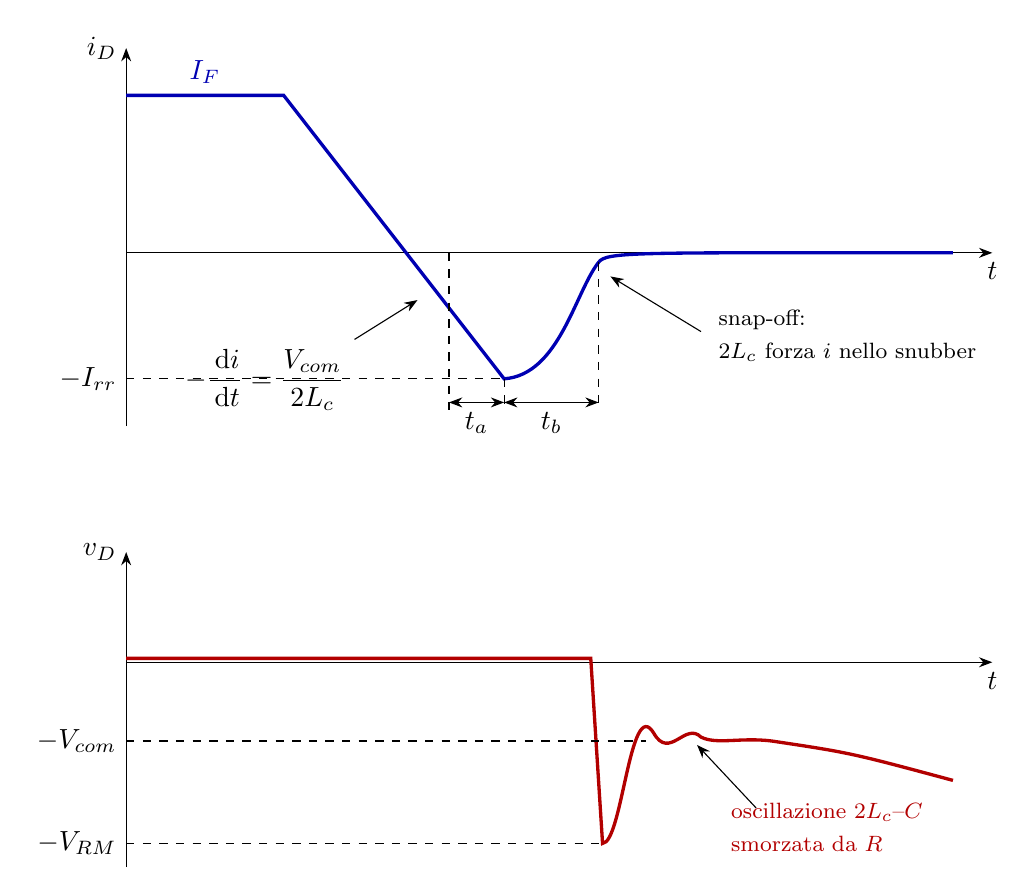
\begin{tikzpicture}[x=1cm, y=1cm, >={Stealth}]
% ---------------- current plot ----------------
\draw[->] (0,0) -- (11,0) node[below] {$t$};
\draw[->] (0,-2.2) -- (0,2.6) node[left] {$i_D$};
% current: on-state, ramp down, undershoot, recovery
\draw[very thick, blue!70!black]
 (0,2) -- (2,2)                      % conduction
 -- (4.8,-1.6)                       % -di/dt, down to -Irr
 .. controls (5.5,-1.55) and (5.7,-0.5) .. (6.0,-0.12)  % tb recovery
 .. controls (6.1,0.02) and (6.5,0) .. (10.5,0);
% annotations
\draw[dashed] (4.1,0) -- (4.1,-2.0);
\draw[dashed] (4.8,-1.6) -- (4.8,-2.0);
\draw[dashed] (6.0,-0.12) -- (6.0,-2.0);
\draw[<->] (4.1,-1.9) -- node[below] {$t_a$} (4.8,-1.9);
\draw[<->] (4.8,-1.9) -- node[below] {$t_b$} (6.0,-1.9);
\draw[dashed] (0,-1.6) node[left] {$-I_{rr}$} -- (4.8,-1.6);
\node[blue!70!black] at (1.0,2.3) {$I_F$};
\draw[<-] (3.7,-0.6) -- (2.9,-1.1) node[below left] {$-\dfrac{\ud i}{\ud t}=\dfrac{V_{com}}{2L_c}$};
\node[align=left, anchor=west] at (7.4,-1.05) {\footnotesize snap-off:\\ \footnotesize $2L_c$ forza $i$ nello snubber};
\draw[->] (7.3,-1.0) -- (6.15,-0.3);
% ---------------- voltage plot ----------------
\begin{scope}[yshift=-5.2cm]
\draw[->] (0,0) -- (11,0) node[below] {$t$};
\draw[->] (0,-2.6) -- (0,1.4) node[left] {$v_D$};
% voltage: ~0 while conducting/recovering, spike at snap, settle to -vll
\draw[very thick, red!70!black]
 (0,0.05) -- (5.9,0.05)
 -- (6.05,-2.3)                       % spike
 .. controls (6.3,-2.3) and (6.4,-0.4) .. (6.7,-0.9)
 .. controls (6.9,-1.25) and (7.1,-0.75) .. (7.3,-0.95)
 .. controls (7.5,-1.05) and (7.8,-0.95) .. (8.2,-1.0)
 .. controls (9.2,-1.15) .. (10.5,-1.5);
\draw[dashed] (0,-2.3) node[left] {$-V_{RM}$} -- (6.05,-2.3);
\draw[dashed] (0,-1.0) node[left] {$-V_{com}$} -- (6.6,-1.0);
\node[red!70!black, align=left] at (8.9,-2.1) {\footnotesize oscillazione $2L_c$--$C$\\ \footnotesize smorzata da $R$};
\draw[->] (8.0,-1.85) -- (7.25,-1.05);
\end{scope}
\end{tikzpicture}
\caption{Corrente e tensione del diodo uscente alla fine della
commutazione. La sovratensione $V_{RM}$ si sviluppa allo snap-off della
corrente di recovery; con snubber RC il transitorio \`e un'oscillazione
smorzata attorno all'inviluppo della tensione concatenata.}
\label{fig:waveforms}
\end{figure}

%=====================================================================
\section{Analisi dello snubber RC}
\label{sec:analisi}

\subsection{Circuito equivalente al momento dello snap-off}

Con lo snubber RC in parallelo al diodo, al momento dello snap-off il
circuito equivalente \`e un RLC serie (fig.~\ref{fig:rlc}): generatore
$V_{com}$ (la concatenata varia poco sulla scala dei $\mathrm{\mu s}$ del
transitorio), induttanza $2L_c$, e la serie $R$--$C$ al posto del diodo
ormai interdetto. Le condizioni iniziali sono
\begin{equation}
i_L(0)=I_{rr}, \qquad v_C(0)\simeq 0,
\end{equation}
perch\'e durante conduzione e recovery la tensione ai capi del diodo (e
quindi del condensatore) \`e trascurabile. La tensione sul diodo \`e
\begin{equation}
v_D(t) = v_C(t) + R\,i(t),
\end{equation}
un'oscillazione smorzata con
\begin{equation}
Z_0 = \sqrt{\frac{2L_c}{C}}, \qquad
\omega_0 = \frac{1}{\sqrt{2L_c\,C}}, \qquad
\zeta = \frac{R}{2 Z_0}.
\label{eq:parametri}
\end{equation}

\begin{figure}[htb]
\centering
\begin{circuitikz}[american, scale=0.95, transform shape]
\ctikzset{bipoles/length=1.0cm}
\draw (0,0) to[V, l=$V_{com}$] (0,3)
      to[L, l=$2L_c$, i>^={$i(0){=}I_{rr}$}] (4,3) -- (5.5,3)
      to[R, l=$R$] (5.5,1.8)
      to[C, l=$C$, v=$v_C$] (5.5,0.6) -- (5.5,0) -- (0,0);
\draw (7.2,3) to[full diode, mirror] (7.2,0);
\node[anchor=east] at (7.0,0.7) {$D$ (off)};
\draw (5.5,3) -- (7.2,3);
\draw (5.5,0) -- (7.2,0);
\draw[<->, thick] (8.3,2.6) -- node[right] {$v_D = v_C + R\,i$} (8.3,0.4);
\end{circuitikz}
\caption{Circuito equivalente del transitorio di snap-off: RLC serie con
corrente iniziale $I_{rr}$ nell'induttanza e condensatore scarico.}
\label{fig:rlc}
\end{figure}

\subsection{Il doppio ruolo di $R$ e il compromesso}

I due contributi alla sovratensione sono ben separabili:
\begin{itemize}
\item \textbf{Salto iniziale resistivo.} All'istante dello snap-off tutta
la $I_{rr}$ viene deviata nello snubber, quindi il diodo vede
istantaneamente
\begin{equation}
\Delta V(0^+) = R\,I_{rr}.
\label{eq:IRstep}
\end{equation}
Una $R$ troppo grande crea da sola lo spike che si voleva evitare.
\item \textbf{Overshoot oscillatorio.} Con $R$ piccola il circuito \`e
poco smorzato e l'energia $E_L$ carica il condensatore ben oltre
$V_{com}$; il limite non smorzato \`e
\begin{equation}
\Delta V_{osc} \le I_{rr}\,Z_0 \quad (\text{caso } R=0,\; v_C(0)=0
\text{ e trascurando il contributo di } V_{com}),
\end{equation}
con oscillazioni prolungate che stressano il condensatore e producono
EMI.
\end{itemize}
Il picco effettivo $V_{RM}$ \`e quindi, in prima approssimazione,
\begin{equation}
V_{RM} \simeq V_{com} + \max\!\big(R\,I_{rr},\; k(\zeta)\, I_{rr} Z_0\big),
\qquad k(\zeta) < 1 \text{ per } \zeta \gtrsim 0{,}4,
\label{eq:VRM_stima}
\end{equation}
e il progetto ottimo bilancia i due termini. Il trattamento rigoroso \`e
quello classico di McMurray \cite{mcmurray}, che parametrizza il problema
con il fattore di corrente iniziale
\begin{equation}
\chi = \frac{I_{rr}\,Z_0}{V_{com}}
\end{equation}
e fornisce curve di progetto per lo smorzamento ottimo e il picco
risultante. Per il caso tipico dei raddrizzatori di linea ($\chi$ elevato,
transitorio dominato dalla corrente) una regola pratica robusta \`e:
\begin{equation}
\boxed{\;
R \simeq (1 \div 1{,}4)\,Z_0
\qquad\Longleftrightarrow\qquad
\zeta \simeq 0{,}5 \div 0{,}7
\;}
\label{eq:Rrule}
\end{equation}
che d\`a un transitorio quasi criticamente smorzato con
$\Delta V \approx (0{,}8\div 1)\,I_{rr}Z_0$ sopra $V_{com}$. Il valore
finale va comunque verificato in simulazione (con modello del diodo
comprensivo di recovery, per esempio Lauritzen--Ma) e poi in collaudo.

\subsection{Dimensionamento di $C$ dal bilancio energetico}

Il condensatore deve assorbire $E_L$ contenendo l'incremento di tensione
entro un $\Delta V_C$ assegnato dal budget di tensione del diodo:
\begin{equation}
\tfrac{1}{2} C\,\Delta V_C^2 \ge \tfrac{1}{2}(2L_c) I_{rr}^2
\qquad\Longrightarrow\qquad
\boxed{\;
C \ge 2L_c \left(\frac{I_{rr}}{\Delta V_C}\right)^{\!2}
\;}
\label{eq:Crule}
\end{equation}
Il budget si costruisce a ritroso da $V_{RRM}$: si fissa il picco
ripetitivo ammesso in esercizio (tipicamente
$V_{RM} \le 0{,}5\div0{,}6\,V_{RRM}$ per lasciare margine ai transitori di
rete non ripetitivi, coordinati con i MOV) e si sottrae $V_{com}$.

\emph{Questo \`e il senso dell'``allineamento'' con l'induttanza di
linea}: $C$ scala linearmente con $L_c$ a parit\`a di $I_{rr}$
(eq.~\ref{eq:Crule}), $R$ scala con $Z_0=\sqrt{2L_c/C}$
(eq.~\ref{eq:Rrule}), e la stessa $I_{rr}$ dipende da $L_c$ attraverso il
$di/dt$ (eq.~\ref{eq:didt_off}--\ref{eq:Irr}). Uno snubber copiato da
un'installazione con trasformatore diverso, o riutilizzato dopo un
potenziamento della rete a monte, non \`e pi\`u dimensionato.

%=====================================================================
\section{Esempio numerico: ponte 690 V / 4 kA}
\label{sec:esempio}

\subsection{Dati di partenza}

\begin{center}
\begin{tabular}{lll}
\toprule
Grandezza & Valore & Note \\
\midrule
Rete & $V_{ll}=690\unit{V}$, $50\unit{Hz}$ & $\hat{V}_{ll}=976\unit{V}$ \\
Corrente DC & $I_d = 4000\unit{A}$ & \\
Trasformatore & $S_n = 4{,}5\unit{MVA}$, $u_k = 6\,\%$ & dedicato \\
Induttanza di commutazione & $L_c \simeq 20\unit{\mu H}$ & da eq.~\eqref{eq:Lc} \\
Diodi & classe $2800\unit{V}$, press-pack & $I_{F(AV)}\simeq1330\unit{A}$/ramo \\
Carica di recovery & $Q_{rr} \simeq 2000\unit{\mu C}$ & a $T_{vj,max}$, dal datasheet \\
Softness & $S \simeq 0{,}3$ & diodo soft \\
\bottomrule
\end{tabular}
\end{center}

Verifica di \eqref{eq:Lc}:
$Z_b = V_{ll}^2/S_n = 690^2/4{,}5\cdot10^6 = 106\unit{m\Omega}$,
$X_c = 0{,}06 \cdot 106 = 6{,}35\unit{m\Omega}$,
$L_c = X_c/\omega = 20{,}2\unit{\mu H}$.

\subsection{Commutazione}

Dall'eq.~\eqref{eq:mu}:
\begin{equation}
\cos\mu = 1 - \frac{2\cdot 314 \cdot 20\cdot10^{-6}\cdot 4000}{976}
        = 1 - 0{,}0515 = 0{,}9485
\;\;\Rightarrow\;\; \mu = 18{,}5^\circ .
\end{equation}
Tensione di commutazione allo spegnimento e $di/dt$
(eq.~\ref{eq:didt_off}):
\begin{equation}
V_{com} = 976 \cdot \sin 18{,}5^\circ \simeq 310\unit{V},
\qquad
\left.\frac{\ud i}{\ud t}\right|_{off}
= \frac{310}{40\unit{\mu H}} \simeq 7{,}7\unit{A/\mu s}.
\end{equation}

\subsection{Reverse recovery}

Dall'eq.~\eqref{eq:Irr}, con $Q_{rr}=2\unit{mC}$ letto sulla curva di
datasheet a $7{,}7\unit{A/\mu s}$ e $T_{vj,max}$:
\begin{equation}
I_{rr} \simeq \sqrt{\frac{2 \cdot 2\cdot10^{-3}\cdot 7{,}7\cdot10^{6}}{1{,}3}}
\simeq 155\unit{A},
\qquad
t_a = \frac{I_{rr}}{\ud i/\ud t} \simeq 20\unit{\mu s},
\quad t_{rr} \simeq 26\unit{\mu s}.
\end{equation}
Energia del loop (eq.~\ref{eq:EL} o, equivalentemente,
\ref{eq:EL_elegante}):
\begin{equation}
E_L = \tfrac{1}{2}\cdot 40\cdot10^{-6}\cdot 155^2 \simeq 0{,}48\unit{J}
\qquad\Big(= \frac{Q_{rr} V_{com}}{1+S}
= \frac{2\cdot10^{-3}\cdot 310}{1{,}3} \simeq 0{,}48\unit{J}\Big).
\end{equation}
Senza snubber, con $C_j \sim 2\unit{nF}$, l'overshoot sarebbe
$I_{rr}\sqrt{2L_c/C_j} \approx 155\cdot\sqrt{40\,\mathrm{\mu H}/2\,\mathrm{nF}}
\approx 22\unit{kV}$ (ovviamente il diodo andrebbe in valanga molto
prima): il fenomeno \`e distruttivo, non un dettaglio.

\subsection{Budget di tensione e scelta di $C$}

Diodo di classe $V_{RRM}=2800\unit{V}$; picco ripetitivo di esercizio
ammesso $V_{RM} \le 1400\unit{V}$ ($=0{,}5\,V_{RRM}$). Poich\'e lo spike
avviene con $V_{com}\simeq310\unit{V}$, il margine disponibile \`e ampio;
si sceglie prudenzialmente un obiettivo di overshoot
$\Delta V_C = 450\unit{V}$ (che tiene conto di tolleranze, dispersione di
$Q_{rr}$ e induttanze parassite non modellate). Dall'eq.~\eqref{eq:Crule}:
\begin{equation}
C \ge 40\cdot10^{-6}\left(\frac{155}{450}\right)^{\!2} \simeq 4{,}7\unit{\mu F}
\qquad\Rightarrow\qquad \boxed{C = 4{,}7\unit{\mu F}}
\end{equation}

\subsection{Scelta di $R$}

\begin{equation}
Z_0 = \sqrt{\frac{40\cdot10^{-6}}{4{,}7\cdot10^{-6}}} \simeq 2{,}9\unit{\Omega},
\qquad
R = 3{,}3\unit{\Omega} \;\Rightarrow\; \zeta = \frac{3{,}3}{2\cdot2{,}9}\simeq 0{,}57.
\end{equation}
Verifiche incrociate:
\begin{itemize}
\item salto resistivo iniziale: $R\,I_{rr} = 3{,}3\cdot155 \simeq 510\unit{V}$;
\item limite oscillatorio non smorzato: $I_{rr}Z_0 \simeq 450\unit{V}$;
\item stima conservativa del picco (eq.~\ref{eq:VRM_stima}):
$V_{RM} \lesssim 310 + 500 \approx 0{,}8\unit{kV}$; la simulazione del
transitorio (\S\ref{sec:verifica}) d\`a $V_{RM} = 575\unit{V}$.
Margine su $V_{RRM}$: $\approx 5\times$.
\end{itemize}
Frequenza propria del transitorio:
$f_0 = 1/(2\pi\sqrt{2L_c C}) \simeq 11{,}6\unit{kHz}$, con costante di
smorzamento di poche decine di $\mathrm{\mu s}$: l'oscillazione si
esaurisce ben prima della commutazione successiva.

\subsection{Perdite e dimensionamento termico di $R$}

In un ponte \emph{a diodi} (a differenza di quello a tiristori) la
tensione di blocco evolve con continuit\`a --- le commutazioni iniziano
allo zero della concatenata, non ci sono gradini di tensione legati
all'angolo di innesco --- quindi le perdite dello snubber sono dominate
dagli eventi di recovery, uno per diodo per ciclo di rete:
\begin{itemize}
\item energia per evento dissipata in $R$: circa
$E_L + \tfrac{1}{2}C V_{com}^2
\simeq 0{,}48 + \tfrac{1}{2}\cdot4{,}7\cdot10^{-6}\cdot310^2
\simeq 0{,}70\unit{J}$;
\item potenza: $P_{rec} \simeq 0{,}70 \cdot 50 \simeq 35\unit{W}$;
\item inseguimento della forma d'onda a frequenza di rete:
$i_C = C\,|\ud v_D/\ud t| \lesssim C\,\omega\hat{V}_{ll} \simeq 1{,}4\unit{A}$,
che in $R$ dissipa pochi watt.
\end{itemize}
In totale $P_R \approx 40\unit{W}$ per snubber: si sceglie un resistore da
$100\unit{W}$ su dissipatore. Sei snubber dissipano
$\approx 250\unit{W}$, irrilevanti sul rendimento di un ponte da
$3{,}6\unit{MW}$ ma da smaltire termicamente nel quadro.

\subsection{Riepilogo}

\begin{center}
\begin{tabular}{lll}
\toprule
Elemento & Valore & Specifica \\
\midrule
$C$ & $4{,}7\unit{\mu F}$ & film PP, $\ge 1600\unit{V_{DC}}$, pulse-rated, ESL bassa \\
$R$ & $3{,}3\unit{\Omega}$ & $\ge 100\unit{W}$, costruzione non induttiva \\
$V_{RM}$ & $575\unit{V}$ (simulazione) & vs. $V_{RRM}=2{,}8\unit{kV}$; stima conservativa $0{,}8\unit{kV}$ \\
$f_0$, $\zeta$ & $11{,}6\unit{kHz}$, $0{,}57$ & transitorio ben smorzato \\
$P_R$ & $\approx 40\unit{W}$/snubber & dominata dagli eventi di recovery \\
\bottomrule
\end{tabular}
\end{center}

Il condensatore lavora in regime con picchi ripetitivi pari al picco della
concatenata ($\approx 976\unit{V}$) pi\`u gli overshoot di recovery: la
scelta di $1600\unit{V_{DC}}$ (o $2000\unit{V_{DC}}$) con adeguato rating
in corrente impulsiva \`e obbligata; i condensatori metallizzati
autocicatrizzanti per snubber sono lo standard.

%=====================================================================
\section{Verifica numerica del transitorio}
\label{sec:verifica}

\subsection{Modello}

Il transitorio di snap-off \`e stato simulato con il modello RLC di
fig.~\ref{fig:rlc}: stato $[i_L,\; v_C]$, condizioni iniziali
$i_L(0)=I_{rr}$, $v_C(0)=0$, generatore $V_{com}$ costante,
$v_D = v_C + R\,i_L$. Lo snap-off ideale (tutta la $I_{rr}$ deviata
istantaneamente nello snubber) \`e il caso di riferimento conservativo
usato da McMurray \cite{mcmurray} e da Mohan \cite{mohan}; un diodo con
coda soft d\`a un picco pi\`u basso a parit\`a di valori. Lo script MATLAB
\`e riportato nell'appendice~\ref{app:matlab}.

\subsection{Progetto scelto}

Con $2L_c = 40\unit{\mu H}$, $V_{com}=310\unit{V}$, $I_{rr}=155\unit{A}$,
$C=4{,}7\unit{\mu F}$, $R=3{,}3\unit{\Omega}$:
\begin{equation}
V_{RM} = 575\unit{V} \quad (t \simeq 8{,}5\unit{\mu s}),
\qquad
V_{RM}-V_{com} = 265\unit{V} \simeq 0{,}58\, I_{rr} Z_0 .
\end{equation}
La stima analitica di $0{,}8\unit{kV}$ (eq.~\ref{eq:VRM_stima}) \`e quindi
conservativa di circa il 40\,\%: i due contributi $R\,I_{rr}$ e
$I_{rr}Z_0$ non si sommano, perch\'e quando il termine resistivo \`e al
massimo il condensatore \`e ancora scarico e viceversa.

\subsection{Sweep di $R$ a $C$ fissata}

La fig.~\ref{fig:sweepR} mostra $V_{RM}(R)$ per $C=4{,}7\unit{\mu F}$. Il
minimo \`e piatto tra $2{,}5$ e $3{,}5\unit{\Omega}$, cio\`e attorno a
$Z_0 = 2{,}9\unit{\Omega}$ ($\zeta \simeq 0{,}4\div0{,}6$): sotto
$2\unit{\Omega}$ il picco risale per sotto-smorzamento, sopra
$4\unit{\Omega}$ cresce quasi linearmente perch\'e domina il salto
$R\,I_{rr}$ (a $10\unit{\Omega}$ si superano $1{,}5\unit{kV}$, con un
$R$ ``troppo prudente'' si costruisce da soli lo spike). La regola
\eqref{eq:Rrule} \`e confermata, e la scelta $R = 3{,}3\unit{\Omega}$
sta nel fondo piatto della curva.

\begin{figure}[htb]
\centering
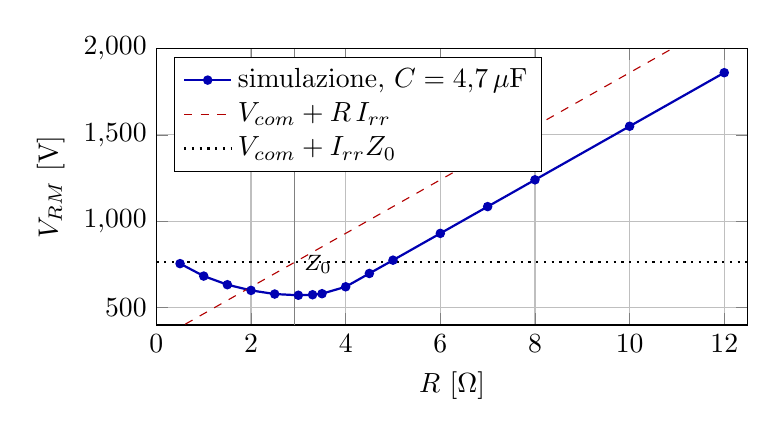
\begin{tikzpicture}
\begin{axis}[width=0.75\textwidth, height=0.42\textwidth,
  xlabel={$R$ [$\Omega$]}, ylabel={$V_{RM}$ [V]},
  xmin=0, xmax=12.5, ymin=400, ymax=2000, grid=major,
  legend pos=north west, legend cell align=left]
\addplot[thick, blue!70!black, mark=*, mark size=1.3pt] coordinates {
 (0.5,755) (1,683) (1.5,633) (2,600) (2.5,579) (3,572) (3.3,575) (3.5,581)
 (4,621) (4.5,698) (5,775) (6,930) (7,1085) (8,1240) (10,1550) (12,1860)};
\addlegendentry{simulazione, $C=4{,}7\,\mu$F}
\addplot[dashed, red!70!black, domain=0:12.5] {310 + 155*x};
\addlegendentry{$V_{com}+R\,I_{rr}$}
\addplot[dotted, thick, black, domain=0:12.5] {310 + 155*2.92};
\addlegendentry{$V_{com}+I_{rr}Z_0$}
\draw[gray, thin] (axis cs:2.92,400) -- (axis cs:2.92,2000)
   node[pos=0.22, right, black] {\footnotesize $Z_0$};
\end{axis}
\end{tikzpicture}
\caption{Picco di tensione sul diodo in funzione di $R$ a
$C=4{,}7\unit{\mu F}$ ($2L_c=40\unit{\mu H}$, $V_{com}=310\unit{V}$,
$I_{rr}=155\unit{A}$). Le rette tratteggiate sono i due termini
asintotici dell'eq.~\eqref{eq:VRM_stima}.}
\label{fig:sweepR}
\end{figure}

\subsection{Sweep di $C$ con $R=Z_0$}

\begin{center}
\begin{tabular}{cccccc}
\toprule
$C$ [$\mu$F] & $R=Z_0$ [$\Omega$] & $V_{RM}$ [V] & $V_{RM}-V_{com}$ [V] &
$f_0$ [kHz] & $P_{rec}\simeq(E_L+\tfrac12 C V_{com}^2)f$ [W] \\
\midrule
1,0  & 6,3 & 1034 & 724 & 25,2 & 27 \\
2,2  & 4,3 & 742  & 432 & 17,0 & 30 \\
3,3  & 3,5 & 640  & 330 & 13,9 & 32 \\
\textbf{4,7} & \textbf{2,9} & \textbf{572} & \textbf{262} & \textbf{11,6} & \textbf{35} \\
6,8  & 2,4 & 519  & 209 & 9,7  & 40 \\
10   & 2,0 & 479  & 169 & 8,0  & 48 \\
15   & 1,6 & 451  & 141 & 6,5  & 60 \\
\bottomrule
\end{tabular}
\end{center}

Oltre $4{,}7\unit{\mu F}$ i rendimenti decrescono: raddoppiare $C$
riduce l'overshoot di un terzo ma aumenta le perdite, il volume e la
corrente impulsiva sul condensatore. Nel caso del ponte a diodi, dove
$V_{com}$ \`e bassa e il margine su $V_{RRM}$ \`e ampio, si potrebbe anche
scendere a $2{,}2\div3{,}3\unit{\mu F}$ con $V_{RM}$ ancora ben sotto
$1\unit{kV}$; $4{,}7\unit{\mu F}$ \`e una scelta con margine per
tolleranze, invecchiamento del condensatore e $Q_{rr}$ reale a caldo.

\subsection{Controllo con la normalizzazione di Mohan}

Mohan \cite{mohan} normalizza il problema con
\begin{equation}
C_{base} = 2L_c\left(\frac{I_{rr}}{V_{com}}\right)^{\!2} = 10\unit{\mu F},
\qquad
R_{base} = \frac{V_{com}}{I_{rr}} = 2{,}0\unit{\Omega},
\end{equation}
e riporta che, per $C = C_{base}$, il picco minimo vale
$V_{max}/V_{com} \simeq 1{,}5$ e si ottiene per $R \simeq 1{,}3\,R_{base}$.
La simulazione con $C=10\unit{\mu F}$ e $R=2{,}6\unit{\Omega}$ d\`a
$V_{max}/V_{com} = 1{,}51$: il modello riproduce le curve di
riferimento. Il progetto scelto corrisponde a $C = 0{,}47\,C_{base}$ e
$R = 1{,}65\,R_{base}$, un punto della mappa spostato verso perdite
minori a fronte di un overshoot relativo maggiore ($1{,}85\,V_{com}$
anzich\'e $1{,}5\,V_{com}$), accettabile perch\'e $V_{com}$ \`e piccola
rispetto alla classe del diodo.

%=====================================================================
\section{Confronto con il ponte a tiristori}
\label{sec:tiristori}

\subsection{Cosa cambia}

Nel ponte a tiristori la commutazione non inizia allo zero della
concatenata ma con ritardo $\alpha$, quindi con tensione di comando
$\hat{V}_{ll}\sin\alpha$ gi\`a applicata. L'angolo di sovrapposizione
segue da
\begin{equation}
\cos\alpha - \cos(\alpha+\mu) = \frac{2\,\omega L_c\, I_d}{\sqrt{2}\,V_{ll}},
\end{equation}
e la tensione di commutazione allo spegnimento del tiristore uscente
diventa
\begin{equation}
V_{com} = \hat{V}_{ll}\sin(\alpha+\mu),
\qquad
\left.\frac{\ud i}{\ud t}\right|_{off} = \frac{\hat{V}_{ll}\sin(\alpha+\mu)}{2L_c}.
\end{equation}
Per $\alpha \to 90^\circ$ (tensione continua media nulla, tipico del
funzionamento a corrente controllata su carichi induttivi, o del
transitorio di avviamento) $V_{com}\to\hat{V}_{ll}$: sia il $di/dt$ sia
la tensione su cui si sovrappone lo spike crescono di un fattore
$\simeq 1/\sin\mu_{diodi}$, oltre $3\times$ nel nostro esempio. Poich\'e
$E_L = Q_{rr}V_{com}/(1+S)$ e $Q_{rr}$ cresce con il $di/dt$, l'energia
dello spike sale per entrambe le vie.

\subsection{Esempio numerico ad $\alpha = 90^\circ$}

Stessa rete ($L_c = 20\unit{\mu H}$), stessa corrente, $Q_{rr}$ scalata
dal valore a $7{,}7\unit{A/\mu s}$ con la dipendenza approssimata
$Q_{rr}\propto\sqrt{di/dt}$ (da sostituire con la curva del datasheet
del tiristore):

\begin{center}
\begin{tabular}{lccc}
\toprule
 & Ponte a diodi & Tiristori, $\alpha=90^\circ$ & Rapporto \\
\midrule
$\mu$ & $18{,}5^\circ$ & $3{,}0^\circ$ & \\
$V_{com}$ & $310\unit{V}$ & $975\unit{V}$ & $3{,}1$ \\
$di/dt$ allo spegnimento & $7{,}7\unit{A/\mu s}$ & $24{,}4\unit{A/\mu s}$ & $3{,}2$ \\
$Q_{rr}$ (a $T_{vj,max}$) & $2{,}0\unit{mC}$ & $\approx3{,}5\unit{mC}$ & $1{,}8$ \\
$I_{rr}$ & $155\unit{A}$ & $365\unit{A}$ & $2{,}4$ \\
$E_L$ per commutazione & $0{,}48\unit{J}$ & $2{,}7\unit{J}$ & $5{,}5$ \\
$V_{RM}$ con $4{,}7\unit{\mu F}/3{,}3\unit{\Omega}$ (sim.) & $575\unit{V}$ & $1540\unit{V}$ & $2{,}7$ \\
$V_{RM}$ con $1\unit{\mu F}/6{,}3\unit{\Omega}$ (sim.) & $1030\unit{V}$ & $2540\unit{V}$ & \\
Energia scaricata da $C$ all'innesco & --- & $\tfrac12 C\hat{V}_{ll}^2 = 2{,}2\unit{J}$ & \\
\bottomrule
\end{tabular}
\end{center}

Lo snubber dimensionato per il ponte a diodi porterebbe il tiristore a
$1{,}54\unit{kV}$, cio\`e a $0{,}55\,V_{RRM}$ per un componente da
$2800\unit{V}$: al limite del budget ripetitivo, senza pi\`u riserva per
i transitori di rete. Con uno snubber ``da tiristori'' di taglia
classica ($1\unit{\mu F}$) si andrebbe a $2{,}5\unit{kV}$, inaccettabile
con quella classe di tensione.

\subsection{Vincoli aggiuntivi del tiristore}

Oltre alla sovratensione di recovery, nel ponte a tiristori lo snubber
deve soddisfare tre vincoli che nel ponte a diodi non esistono:
\begin{enumerate}
\item \textbf{$dv/dt$ critico.} Un $dv/dt$ riapplicato eccessivo
(subito dopo il recovery sul tiristore uscente, oppure per gradini di
tensione sui tiristori in blocco causati dagli inneschi degli altri
rami) pu\`o innescare spuriamente il componente. Il rating tipico dei
tiristori da fase \`e $500\div1000\unit{V/\mu s}$: il salto $R\,I_{rr}$,
praticamente istantaneo, va tenuto basso, il che spinge verso $R$
piccola e $C$ grande.
\item \textbf{Scarica di $C$ all'innesco.} All'accensione il tiristore
cortocircuita lo snubber carico a $\hat{V}_{ll}\sin\alpha$: la corrente
di scarica $\hat{V}_{ll}\sin\alpha/R$ (con $3{,}3\unit{\Omega}$ e
$\alpha=90^\circ$, $\simeq 300\unit{A}$, con $di/dt$ limitato solo dai
parassiti del loop snubber) si somma al $di/dt$ di carico e deve
rispettare il $di/dt$ critico e la capacit\`a di comando del gate. Questo
vincolo spinge verso $R$ \emph{grande}, in conflitto con il precedente.
\item \textbf{Perdite.} Ogni innesco dissipa in $R$ l'energia
$\tfrac12 C(\hat{V}_{ll}\sin\alpha)^2$ ($2{,}2\unit{J}$, cio\`e
$110\unit{W}$ a $50\unit{Hz}$ con $4{,}7\unit{\mu F}$), e ogni gradino
di tensione sui rami in blocco altrettanto ($\tfrac12 C\Delta V^2$ per
gradino, indipendentemente da $R$). Complessivamente
$P_R \approx k\,f\,C\,\hat{V}_{ll}^2$ con $k\simeq1\div3$ secondo
$\alpha$: con $4{,}7\unit{\mu F}$ si arriva a diverse centinaia di watt
per snubber, contro i $\approx40\unit{W}$ del ponte a diodi.
\end{enumerate}

\subsection{Conseguenze progettuali}

Il problema del ponte a diodi \`e ``economico'' perch\'e $V_{com}$ \`e
piccola: si pu\`o comprare il margine con $C$ generosa a costo
trascurabile. Nel ponte a tiristori l'angolo critico
($\alpha\simeq90^\circ$ a corrente nominale) rende la stessa strategia
costosa in perdite, e il progetto diventa un compromesso a pi\`u
variabili: capacit\`a pi\`u piccola ($0{,}25\div1\unit{\mu F}$) e $R$
maggiore ($10\div50\unit{\Omega}$) accettando un overshoot relativo pi\`u
alto, classe di tensione superiore o soft-recovery spinto, e in
parallelo dispositivi di clamp di ponte (RC lato DC, MOV lato AC) che
assorbono parte dell'energia di commutazione. La verifica va fatta
sull'intero campo di $\alpha$, non solo al punto nominale: ad
$\alpha\to0$ il ponte a tiristori si comporta come quello a diodi, ma
\`e al centro del campo di regolazione che si trova la condizione
dimensionante.


\label{sec:sensibilita}

Vale la pena rendere esplicita la catena di dipendenze da $L_c$, perch\'e
\`e ci\`o che rende lo snubber specifico dell'installazione:
\begin{itemize}
\item $L_c \downarrow$ (rete pi\`u rigida, es. collegamento diretto a una
sbarra con alta potenza di corto circuito): $\mu\downarrow$ ma
$di/dt \uparrow \;(\propto 1/\sqrt{L_c}$ in prima approssimazione$)$,
quindi $I_{rr}\uparrow$ e $Z_0$ cambia; $R$ e $C$ vanno ricalcolati e il
transitorio diventa pi\`u veloce;
\item $L_c \uparrow$ (trasformatore con $u_k$ maggiore, reattanze
aggiuntive): $di/dt\downarrow$ e $I_{rr}\downarrow$, ma a parit\`a di
$I_{rr}$ serve pi\`u capacit\`a (eq.~\ref{eq:Crule}) e l'energia per
evento si sposta secondo l'eq.~\eqref{eq:EL_elegante};
\item la ripartizione di $L_c$ conta: l'induttanza \emph{interna} al
loop snubber--diodo (sbarre tra capsula e snubber) non \`e coperta dallo
snubber e produce comunque $L_{par}\,\ud i/\ud t$ direttamente sul
silicio. Da qui la regola di montaggio: snubber il pi\`u vicino possibile
al componente, con collegamenti a bassa induttanza (obiettivo
$L_{par} \lesssim$ decine di nH).
\end{itemize}
In pratica: a ogni modifica della rete a monte (nuovo trasformatore,
rifasamento, potenziamento della sbarra) la verifica dello snubber va
ripetuta, idealmente con misura oscillografica di $v_D$ al collaudo.

%=====================================================================
\section{Note pratiche e protezioni complementari}

\begin{itemize}
\item \textbf{Scelta del diodo.} Preferire diodi da raddrizzamento con
recovery dichiaratamente \emph{soft} ($S$ elevato): riducono $I_{rr}$
efficace allo snap e l'ampiezza dello spike a parit\`a di snubber.
\item \textbf{Layout.} Loop snubber--diodo minimo; resistori non
induttivi (a griglia, o a filo con avvolgimento bifilare); condensatori
con terminazioni a bassa ESL, eventualmente due in parallelo per
dimezzare ESL e ripartire la corrente impulsiva.
\item \textbf{MOV.} Varistori sui diodi o sul lato AC coordinano la
protezione contro i transitori di rete non ripetitivi (manovre di
interruttori a monte, fulminazione), che lo snubber RC da solo non
copre: lo snubber gestisce il fenomeno ripetitivo di recovery, il MOV
l'evento raro ad alta energia.
\item \textbf{Verifica sperimentale.} In collaudo misurare $v_D$ con
sonda differenziale ad alta tensione e banda adeguata ($\ge 10\times f_0$)
direttamente sui terminali della capsula, a corrente nominale e macchina
calda: \`e l'unica conferma reale di $V_{RM}$, perch\'e $Q_{rr}$ a caldo e
le induttanze parassite reali sono note solo approssimativamente.
\item \textbf{Simulazione.} Un modello di diodo con recovery fisico (per
esempio Lauritzen--Ma) nel loop con $2L_c$, snubber e parassiti di
montaggio permette di verificare $V_{RM}$, la sensibilit\`a a $Q_{rr}$ e
il de-rating prima del collaudo.
\end{itemize}

%=====================================================================
\section{Conclusioni}

Nel ponte a diodi di alta potenza la sovratensione dimensionante per i
semiconduttori nasce dal reverse recovery in combinazione con
l'induttanza del loop di commutazione $2L_c$: allo snap-off l'energia
$E_L = Q_{rr}V_{com}/(1+S)$ deve trovare un percorso, e senza snubber lo
trova nella capacit\`a di giunzione con overshoot distruttivi. Lo snubber
RC si dimensiona in due passi legati entrambi a $L_c$: il condensatore dal
bilancio energetico $C \ge 2L_c(I_{rr}/\Delta V_C)^2$, il resistore dallo
smorzamento $R \approx (1\div1{,}4)\sqrt{2L_c/C}$, con la verifica che il
salto iniziale $R\,I_{rr}$ non domini il picco. Nell'esempio
$690\unit{V}/4\unit{kA}$ si arriva a valori del tutto tipici
($4{,}7\unit{\mu F}$, $3{,}3\unit{\Omega}$, $\approx40\unit{W}$ per
snubber) con picco simulato $\approx0{,}6\unit{kV}$ contro
$V_{RRM}=2{,}8\unit{kV}$; nel ponte a tiristori lo stesso fenomeno,
valutato ad $\alpha\simeq90^\circ$, \`e circa $5\times$ pi\`u energetico e
si somma ai vincoli di $dv/dt$, di scarica all'innesco e di perdite, che
cambiano radicalmente il compromesso. Il punto di metodo \`e che questi valori non
sono ``dello snubber'' ma \emph{della coppia snubber--rete}: cambiando
l'induttanza di linea, il dimensionamento va rifatto.

%=====================================================================
\appendix
\section{Script MATLAB di verifica}
\label{app:matlab}

Lo script calcola la catena di dimensionamento (induttanza di
commutazione, $\mu$, $di/dt$, $I_{rr}$), simula il transitorio di
snap-off con \texttt{ode45}, stampa $V_{RM}$ e i parametri di Mohan,
stima le perdite ed esegue gli sweep di $R$ e di $C$ dei
\S\ref{sec:verifica}. Con \texttt{alpha\_deg} $>0$ valuta il caso del
ponte a tiristori del \S\ref{sec:tiristori} (parte di recovery, scarica
del condensatore all'innesco e sue perdite). File:
\texttt{snubber\_rlc\_check.m}.

\begin{lstlisting}
%% snubber_rlc_check.m
% RC snubber verification for a high-power three-phase diode bridge.
% Companion to snubber_ponte_diodi.tex.
%
%   1. commutation inductance, overlap angle, di/dt at turn-off
%   2. reverse recovery peak current from Qrr and softness factor
%   3. snap-off transient of the series RLC (2*Lc, R, C) -> VRM
%   4. Mohan normalisation (Cbase, Rbase)
%   5. loss estimate
%   6. R sweep at fixed C, C sweep with R = Z0(C)
%
% The ideal snap-off (all of Irr diverted into the snubber at t = 0,
% capacitor discharged) is the conservative reference case used by
% McMurray (1972) and Mohan. Set alpha_deg > 0 to evaluate a thyristor
% bridge at a given firing angle (recovery part only; dv/dt, firing
% discharge and voltage-step losses are reported as separate figures).

clear; close all; clc;

%% 1. Input data ---------------------------------------------------------
Vll      = 690;       % line-to-line rms voltage [V]
f        = 50;        % grid frequency [Hz]
Id       = 4000;      % DC current [A]
Sn       = 4.5e6;     % transformer rating [VA]
uk       = 0.06;      % transformer short-circuit voltage [p.u.]
Lext     = 0;         % extra line/busbar inductance per phase [H]
Qrr_ref  = 2.0e-3;    % recovery charge from datasheet [C] ...
didt_ref = 7.7e6;     % ... at this di/dt [A/s], Tvj,max
scaleQrr = true;      % scale Qrr ~ sqrt(di/dt) around the reference point
S        = 0.3;       % softness factor tb/ta
C        = 4.7e-6;    % snubber capacitance [F]
R        = 3.3;       % snubber resistance [ohm]
VRRM     = 2800;      % device voltage class [V]
kVRM     = 0.5;       % allowed repetitive peak as a fraction of VRRM
alpha_deg = 0;        % firing angle: 0 = diode bridge, > 0 = thyristor bridge

%% 2. Commutation --------------------------------------------------------
w     = 2*pi*f;
Vpk   = sqrt(2)*Vll;
Zb    = Vll^2/Sn;
Lc    = uk*Zb/w + Lext;                  % commutation inductance per phase [H]
L     = 2*Lc;                            % loop inductance seen by the transient
alpha = alpha_deg*pi/180;
mu    = acos(cos(alpha) - 2*w*Lc*Id/Vpk) - alpha;   % overlap angle [rad]
Vcom  = Vpk*sin(alpha + mu);             % commutation voltage at turn-off [V]
didt  = Vcom/L;                          % di/dt at turn-off [A/s]

%% 3. Reverse recovery ---------------------------------------------------
if scaleQrr
    Qrr = Qrr_ref*sqrt(didt/didt_ref);
else
    Qrr = Qrr_ref;
end
Irr = sqrt(2*Qrr*didt/(1+S));
ta  = Irr/didt;
trr = ta*(1+S);
EL  = 0.5*L*Irr^2;                       % = Qrr*Vcom/(1+S)

%% 4. Snap-off transient -------------------------------------------------
Z0   = sqrt(L/C);
zeta = R/(2*Z0);
f0   = 1/(2*pi*sqrt(L*C));
[t, vD, iL, vC] = snap_transient(Vcom, Irr, L, C, R);
[VRM, kmax] = max(vD);
tVRM = t(kmax);

%% 5. Mohan normalisation ------------------------------------------------
Cbase = L*(Irr/Vcom)^2;
Rbase = Vcom/Irr;

%% 6. Losses -------------------------------------------------------------
% diode bridge: one recovery event per device per cycle; the blocking
% voltage evolves continuously, so no step-induced losses
Erec = EL + 0.5*C*Vcom^2;                % energy dissipated in R per event [J]
Pfol = 0.5*R*(C*w*Vpk)^2;                % waveform-following term, rough bound [W]
PR   = Erec*f + Pfol;
if alpha > 0
    Vfire  = Vpk*sin(alpha);             % device voltage at firing
    Efire  = 0.5*C*Vfire^2;              % capacitor discharge through R at firing
    Idisch = Vfire/R;                    % peak discharge current into the device
    PR     = PR + Efire*f;               % step losses from other legs NOT included
end

%% 7. Report -------------------------------------------------------------
fprintf('--- Commutation ---------------------------------------------\n');
fprintf('Lc = %.1f uH  (2Lc = %.1f uH)\n', Lc*1e6, L*1e6);
fprintf('mu = %.2f deg,  Vcom = %.0f V,  di/dt = %.2f A/us\n', ...
        mu*180/pi, Vcom, didt*1e-6);
fprintf('--- Reverse recovery ----------------------------------------\n');
fprintf('Qrr = %.2f mC,  Irr = %.0f A,  ta = %.1f us,  trr = %.1f us\n', ...
        Qrr*1e3, Irr, ta*1e6, trr*1e6);
fprintf('EL = 0.5*(2Lc)*Irr^2 = %.3f J   (Qrr*Vcom/(1+S) = %.3f J)\n', ...
        EL, Qrr*Vcom/(1+S));
fprintf('--- Snubber -------------------------------------------------\n');
fprintf('C = %.2f uF,  R = %.2f ohm,  Z0 = %.2f ohm,  zeta = %.2f,  f0 = %.1f kHz\n', ...
        C*1e6, R, Z0, zeta, f0*1e-3);
fprintf('R*Irr = %.0f V,  Irr*Z0 = %.0f V\n', R*Irr, Irr*Z0);
if VRM <= kVRM*VRRM, status = 'OK'; else, status = 'FAIL'; end
fprintf('VRM = %.0f V at t = %.1f us  (limit %.0f V = %.2f*VRRM)  -> %s\n', ...
        VRM, tVRM*1e6, kVRM*VRRM, kVRM, status);
fprintf('Mohan: Cbase = %.2f uF, Rbase = %.2f ohm  ->  C/Cbase = %.2f, R/Rbase = %.2f\n', ...
        Cbase*1e6, Rbase, C/Cbase, R/Rbase);
fprintf('--- Losses --------------------------------------------------\n');
fprintf('Energy per recovery event in R = %.2f J  ->  %.0f W\n', Erec, Erec*f);
fprintf('Total P_R = %.0f W per snubber\n', PR);
if alpha > 0
    fprintf('Firing: V = %.0f V, discharge peak = %.0f A, %.2f J -> %.0f W\n', ...
            Vfire, Idisch, Efire, Efire*f);
end

%% 8. R sweep at fixed C -------------------------------------------------
Rvec  = linspace(0.25, 4*Z0, 60);
VRM_R = zeros(size(Rvec));
for n = 1:numel(Rvec)
    [~, v] = snap_transient(Vcom, Irr, L, C, Rvec(n));
    VRM_R(n) = max(v);
end
[VRM_opt, nopt] = min(VRM_R);
fprintf('R sweep: min VRM = %.0f V at R = %.2f ohm (%.2f*Z0)\n', ...
        VRM_opt, Rvec(nopt), Rvec(nopt)/Z0);

%% 9. C sweep with R = Z0(C) --------------------------------------------
Cvec  = logspace(log10(0.5e-6), log10(20e-6), 30);
VRM_C = zeros(size(Cvec));
for n = 1:numel(Cvec)
    [~, v] = snap_transient(Vcom, Irr, L, Cvec(n), sqrt(L/Cvec(n)));
    VRM_C(n) = max(v);
end
Prec_C = (EL + 0.5*Cvec*Vcom^2)*f;

%% 10. Plots -------------------------------------------------------------
figure('Name', 'Snap-off transient');
subplot(2,1,1);
plot(t*1e6, vD, 'LineWidth', 1.5); hold on; grid on;
plot([t(1) t(end)]*1e6, Vcom*[1 1], 'k--');
plot([t(1) t(end)]*1e6, kVRM*VRRM*[1 1], 'r--');
ylabel('v_D [V]');
title(sprintf('C = %.1f uF, R = %.2f ohm: V_{RM} = %.0f V', C*1e6, R, VRM));
legend('v_D', 'V_{com}', 'limit', 'Location', 'best');
subplot(2,1,2);
plot(t*1e6, iL, t*1e6, vC/R, 'LineWidth', 1.2); grid on;
xlabel('t [us]'); ylabel('[A]');
legend('i_L = i_{snubber}', 'v_C / R', 'Location', 'best');

figure('Name', 'Sweeps');
subplot(1,2,1);
plot(Rvec, VRM_R, 'LineWidth', 1.5); hold on; grid on;
plot(Rvec, Vcom + Rvec*Irr, 'r--');
plot([Z0 Z0], [min(VRM_R)*0.9 max(VRM_R)], 'k:');
xlabel('R [ohm]'); ylabel('V_{RM} [V]');
title(sprintf('R sweep, C = %.1f uF', C*1e6));
legend('V_{RM}', 'V_{com} + R I_{rr}', 'Z_0', 'Location', 'northwest');
subplot(1,2,2);
yyaxis left;  semilogx(Cvec*1e6, VRM_C, 'LineWidth', 1.5); ylabel('V_{RM} [V]');
yyaxis right; semilogx(Cvec*1e6, Prec_C, 'LineWidth', 1.2); ylabel('P_{rec} [W]');
grid on; xlabel('C [uF]'); title('C sweep, R = Z_0(C)');

%% Local function --------------------------------------------------------
function [t, vD, iL, vC] = snap_transient(Vcom, I0, L, C, R)
% Series RLC after ideal snap-off: source Vcom, loop inductance L,
% snubber R-C in place of the diode. State x = [iL; vC],
% iL(0) = I0, vC(0) = 0, diode voltage vD = vC + R*iL.
    A    = [-R/L, -1/L; 1/C, 0];
    b    = [Vcom/L; 0];
    w0   = 1/sqrt(L*C);
    zeta = R/2*sqrt(C/L);
    tend = max(8/(max(zeta, 0.05)*w0), 4*2*pi/w0);
    opts = odeset('RelTol', 1e-8, 'AbsTol', 1e-9, 'MaxStep', tend/2000);
    [t, x] = ode45(@(t, x) A*x + b, [0 tend], [I0; 0], opts);
    iL = x(:,1);
    vC = x(:,2);
    vD = vC + R*iL;
end
\end{lstlisting}

%=====================================================================
\begin{thebibliography}{9}

\bibitem{mohan} N.~Mohan, T.~M.~Undeland, W.~P.~Robbins,
\emph{Power Electronics: Converters, Applications, and Design},
3rd ed., Wiley, 2003.

\bibitem{mcmurray} W.~McMurray,
``Optimum snubbers for power semiconductors,''
\emph{IEEE Transactions on Industry Applications},
vol.~IA-8, no.~5, pp.~593--600, 1972.

\bibitem{abb} ABB Switzerland Ltd, Semiconductors,
``Design of RC snubbers for phase control applications,''
Application Note 5SYA~2020.

\bibitem{semikron} A.~Wintrich, U.~Nicolai, W.~Tursky, T.~Reimann,
\emph{Application Manual Power Semiconductors},
2nd ed., SEMIKRON International, 2015.

\bibitem{linder} S.~Linder,
\emph{Power Semiconductors}, EPFL Press, 2006.

\end{thebibliography}

\end{document}
